\section{Evaluation}
\label{sec:evaluation}

\subsection{Experimental Setup}
\label{subsec:experimental-setup}

Experiments are conducted on two NVIDIA GPUs: an A100 SXM4-80GB (108 streaming multiprocessors) and an H20 (78 streaming multiprocessors). The principal workload is the downhole positioning dataset with a $15$-dimensional error state, augmented by batch variants, and the CPU eager fp64 implementation serves as the numerical golden reference. All GPU runs use PyTorch 2.11.0 with CUDA 12.9 and Triton 3.6.0.

All fused kernels are written as a single Triton program. Reported timings exclude kernel compilation and autotuning and use warm-up runs of the same shape as the measured execution; each configuration is timed at least three times after synchronization and the mean is reported. Throughput is reported in filter steps per second throughout, and as aggregate steps per second for batch experiments.

The comparative methods are: (i) \texttt{torch eager}, a per-step tensor implementation using \texttt{torch.linalg.inv}; (ii) \texttt{torch compile}, Inductor auto-fusion of the single-step function (about eighteen dispatches per step); (iii) \textsc{PrefixScan}, a temporal-parallel prefix-sum scan for Bayesian filtering~\cite{sarkka2021temporal}, which combines batched dense matrices through cuBLAS and cuSOLVER; and (iv) \textsc{Trident}, the fused whole-scan Triton kernel of this paper. Method (iii) assumes a linear filtering core and is therefore applied only to the linear workloads of the corresponding experiments.

\subsection{End-to-End Performance}
\label{subsec:end-to-end}

\begin{figure*}[!t]
  \centering
  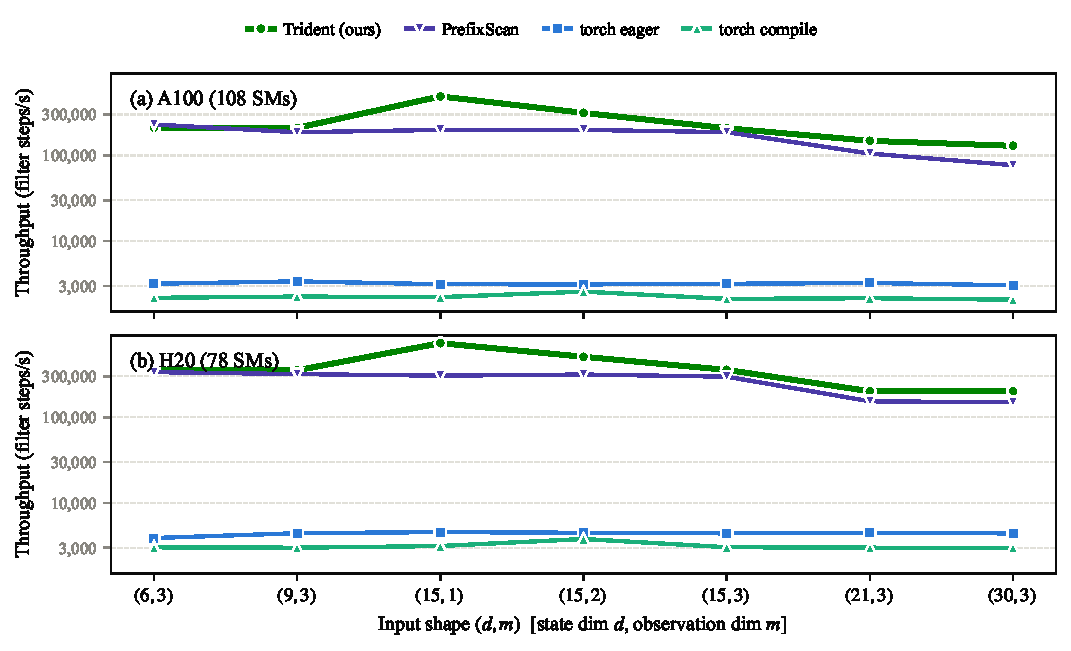
\includegraphics[width=\textwidth]{figures/5-eval-shape.pdf}
  \caption{Throughput of the linear Kalman core as the state dimension $d$ and observation dimension $m$ vary (single trajectory, fp32). (a) A100; (b) H20.}
  \label{fig:shape-compare}
\end{figure*}

On a single trajectory, the fused implementation removes the latency bound that dominates the eager baselines (measured on the H20). The CPU eager fp64 reference sustains $1{,}866$ steps/s; a CUDA Graph replay of the same per-step kernels reaches $2{,}640$ steps/s ($1.41\times$), and whole-scan fusion in fp64 raises this to $16{,}491$ steps/s ($8.8\times$ over the CPU). Switching the fused kernel to the adopted fp32 precision plan reaches $242{,}737$ steps/s, $130\times$ over the CPU reference. Batching independent trajectories then scales the same kernel to $1.9\times10^{7}$ steps/s at 78 trajectories and to a peak of $4.63\times10^{7}$ steps/s at 312 trajectories, approximately $2.5\times10^{4}\times$ the CPU; \Cref{subsec:ablation} analyzes this scaling in detail.

\Cref{fig:shape-compare} generalizes the comparison beyond the end-to-end workload by sweeping the state dimension $d$ and observation dimension $m$ of the linear Kalman core on both GPUs. Two observations hold across the entire sweep. First, the two scan-based implementations outperform the per-step baselines by about two orders of magnitude at every configuration: \texttt{torch eager} and \texttt{torch compile} remain in a narrow $2$--$4.5\times10^{3}$ steps/s band regardless of shape, because their cost is dominated by kernel dispatch rather than arithmetic. Second, \textsc{Trident} is more robust than \textsc{PrefixScan} to both shape directions. Increasing $d$ from 15 to 30 reduces \textsc{PrefixScan} from $1.87\times10^{5}$ to $7.7\times10^{4}$ steps/s on the A100, while \textsc{Trident} retains $1.29\times10^{5}$ steps/s; the H20 panel shows the same ordering. Decreasing $m$ widens the gap in \textsc{Trident}'s favor---at $(d,m)=(15,1)$ it reaches $4.9\times10^{5}$ steps/s on the A100 and $7.3\times10^{5}$ steps/s on the H20, up to $2.3\times$ the corresponding \textsc{PrefixScan} rate---because the analytical innovation inverse removes the cuSOLVER call that the prefix scan requires at every step.

\subsection{Numerical Accuracy Under Mixed Precision}
\label{subsec:precision-evaluation}

We evaluate accuracy on complete trajectories rather than isolated filter steps, because \Cref{subsec:motivation-precision} shows that rounding in recurrent quantities accumulates over the full horizon and a truncated run would understate it. \Cref{tab:precision-fidelity} scores the baselines on the linear Kalman core against a sequential fp64 evaluation of the same filter. All fp32 implementations reproduce that reference to about $10^{-7}$ at the final state, and \textsc{Trident} is the fastest while matching the eager baseline's accuracy grade: $1.8\times$ the \textsc{PrefixScan} throughput and $130\times$ the eager baseline at the same $10^{-7}$ accuracy. Their throughput differences therefore do not come at the cost of accuracy. The only unattractive choice is the TF32 dot product, which degrades by four orders of magnitude to $1.3\times10^{-3}$, confirming the component-aware selection of IEEE dot products in \Cref{subsec:mixed-precision}.

The same ordering holds on the end-to-end SINS/EKF workload, where the filter's own positioning error provides a physical accuracy scale: the adopted fp32 plan deviates from the fp64 CPU reference by only $4.3$\,mm over the complete trajectory---two orders of magnitude below the reference's own $1{,}017.838$\,mm error---while running $130\times$ faster, and the fused fp64 variant deviates by $0.31$\,mm, so the residual error stems from the precision plan rather than from fusion. Applied with the acceptance ratio $\alpha{=}10^{-2}$, the criterion \Cref{eq:precision-accept} admits precision-induced deviations up to $\alpha\,\varepsilon_{\mathrm{model}}\approx10.2$\,mm for this workload---over twice the adopted plan's $4.3$\,mm---so the selection is comfortably within tolerance. Acceleration therefore does not cost accuracy on either workload.

\begin{table}[!t]
  \centering
  \caption{Accuracy and throughput of fp32 implementations on the linear Kalman core, $(d,m)=(15,3)$, single trajectory (A100). $\Delta$ is the final-state deviation $\max|\mathbf{x}-\mathbf{x}^{\mathrm{ref}}|$ from a sequential fp64 evaluation of the same filter.}
  \label{tab:precision-fidelity}
  \begin{tabular}{@{}lrr@{}}
    \toprule
    Implementation & Steps/s & $\Delta$ vs fp64 ref. \\
    \midrule
    \texttt{torch eager} & 2,108 & $1.1\times10^{-7}$ \\
    \textsc{PrefixScan} & 152,932 & $3.0\times10^{-7}$ \\
    \textsc{Trident} (ours) & \textbf{274,428} & $\mathbf{1.2\times10^{-7}}$ \\
    \bottomrule
  \end{tabular}
\end{table}

\subsection{Ablation Study}
\label{subsec:ablation}

We decompose the end-to-end gain of \Cref{subsec:end-to-end} into the three axes of \textsc{Trident} and quantify each axis independently. We first ablate the three contributions against the end-to-end workload, then present Nsight profiling of GPU utilization that connects the observed performance regimes to how the device is actually occupied.

\subsubsection{Axis combination and isolation}
\Cref{fig:ablation-shape} isolates each of the three axes against the eager fp64 GPU baseline on the end-to-end SINS/EKF workload and contrasts them with the full combination. Two observations stand out. First, no single axis suffices: enabling only the fp32 precision plan barely moves the launch-bound eager step ($449\to492$ steps/s), and even batching 108 eager trajectories ($4.4\times10^{4}$ steps/s) loses to a \emph{single} fused fp64 trajectory ($7.1\times10^{4}$ steps/s), because launch-bound execution never reaches the arithmetic that precision or fusion would accelerate. Second, the axes compose multiplicatively rather than additively---fusion $157\times$, precision a further $1.8\times$ on A100, batching $109\times$, whose product ($\approx3.1\times10^{4}\times$) matches the full combination---because each removes a distinct bottleneck: fusion removes dispatch and recurrent-state traffic on the serial critical path, precision shortens per-step arithmetic, and batching fills the SMs a single scan leaves idle. The remaining cells of the $2{\times}2{\times}2$ factorial (measured but omitted from the figure for clarity) confirm that these factors are consistent across conditionings: fusion gains $157$--$311\times$ (rising once the other axes expose arithmetic to it), precision pays only on fused execution ($1.8\times$ at $B{=}1$, $1.24\times$ at $B{=}108$) and is within noise on eager variants, and batching contributes $89$--$157\times$ in every conditioning. Launch-bound variants are invariant to trajectory length, so these conclusions do not depend on the horizon $N{=}166{,}667$.

\begin{figure}[!t]
  \centering
  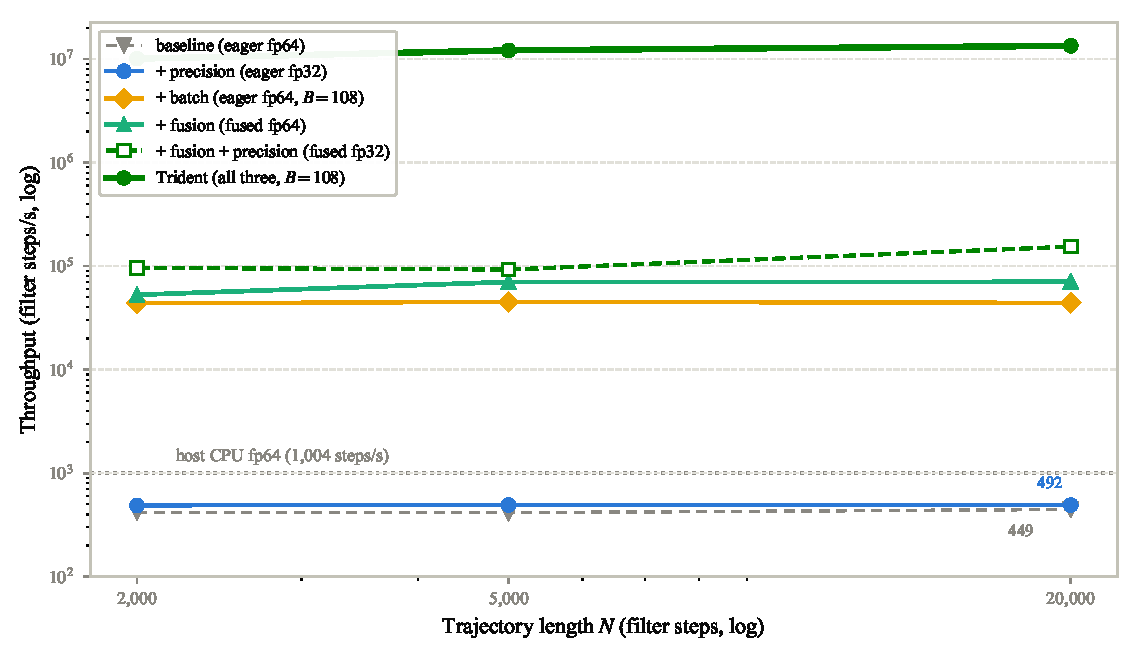
\includegraphics[width=\linewidth]{figures/5-eval-ablation-a100.pdf}
  \caption{Contribution ablation on the end-to-end SINS/EKF workload (A100). Against the eager fp64 GPU baseline, each intermediate series enables exactly one optimization axis in isolation---fusion (fused fp64), the fp32 precision plan (eager fp32), or trajectory batching (eager fp64, $B{=}108$, one per SM)---and \textsc{Trident} enables all three. Because launch-bound implementations are trajectory-length invariant (flat in $N$), all series are shown up to the common horizon $N{=}20{,}000$.}
  \label{fig:ablation-shape}
\end{figure}

\subsubsection{Conditional per-axis gains}
Each axis also carries a caveat that makes its gain conditional rather than automatic. For fusion, the eager tensor port is \emph{slower than the CPU} (263--610 steps/s across $\sim$531 launches per step) and even CUDA Graph replay reaches only $1.41\times$; only enclosing the whole scan in one kernel breaks the latency bound, and a library-composition bound explains why---a cuBLAS $\mathbf{F}\mathbf{P}\mathbf{F}^{\mathsf T}$ plus a cuSOLVER $3\times3$ inverse already cost $2.2\times$ the complete fused step. For precision, the $14.7\times$ on H20 versus only $1.8\times$ on A100: the A100 runs fp64 at half its fp32 rate, so the fp32-over-fp64 ceiling is near $2\times$, whereas on the H20 the fp64 datapath is only a small fraction of the fp32 rate, releasing far greater step-level throughput on the same switch---an asymmetry that motivates the per-device selection of \Cref{subsec:mixed-precision}. The gain on both devices comes from the \emph{selective} assignment: a uniform TF32 plan is both slower ($0.86\times$) and less accurate ($4.82$\,mm) than the adopted fp32/IEEE plan. For batching, \Cref{tab:ablation-batch} shows throughput peaks at $B{=}312$---one full register-limited wave, $186\times$ a single trajectory---and \emph{falls} $24\%$ at $B{=}400$ once wave quantization leaves the second wave only $28\%$ populated, exactly as the register-residency model of \Cref{subsec:batch-parallelism} predicts.


\begin{table}[!t]
  \centering
  \caption{Batch-size sweep of the fused fp32 kernel on H20 (median of repeated runs). Blocks/SM is $B/78$; per-trajectory efficiency normalizes throughput to $B\times$ the $B{=}1$ rate. The $B{=}1$ row corresponds to the fused fp32 configuration of \Cref{subsec:end-to-end}, re-measured as the median of the batch sweep.}
  \label{tab:ablation-batch}
  \begin{tabular}{@{}rrrrl@{}}
    \toprule
    $B$ & Blocks/SM & Steps/s & Efficiency & Regime \\
    \midrule
    1 & 0.01 & 248,159 & 1.000 & linear \\
    8 & 0.10 & 1,959,084 & 0.987 & linear \\
    32 & 0.41 & 7,830,144 & 0.986 & linear \\
    78 & 1.00 & 19,086,444 & 0.986 & one block per SM \\
    96 & 1.23 & 19,954,522 & 0.838 & register co-residency \\
    156 & 2.00 & 32,239,540 & 0.833 & register co-residency \\
    256 & 3.28 & 38,029,702 & 0.599 & register co-residency \\
    312 & 4.00 & 46,290,218 & 0.598 & peak, one full wave \\
    400 & 5.13 & 35,016,136 & 0.353 & oversubscribed \\
    \bottomrule
  \end{tabular}
\end{table}

\subsubsection{Device-utilization profile}
A GPU-utilization profile ties these regimes to how the device is occupied, and \Cref{tab:ablation-profiling} summarizes the measured Nsight counters. Kernel-launch tracing (Nsight Systems) confirms that whole-scan fusion removes the dispatch bottleneck entirely---a full $166{,}667$-step trajectory executes as a single \texttt{ekf\_mega\_kernel\_p} launch---so with no dispatch overhead left, the remaining lever is how much of the device that one launch occupies. Nsight Compute shows the answer for a single trajectory is "very little": one $128$-thread block (four warps) lands on one of $78$ SMs ($\approx1.3\%$ of the device), achieved occupancy on that SM is $6.25\%$ ($4$ of $64$ warps), and device-wide SM throughput is $0.27\%$ (\Cref{tab:motivation-utilization}). This double under-subscription---few SMs among many, few warps within the active one---is the quantitative root of the latency-bound behavior.

\subsubsection{Register-limited batch scaling}
Batch-level mapping closes exactly this gap. At $B{=}78$ the grid places one block on every SM and measured SM throughput rises $74\times$, from $0.27\%$ to $19.91\%$, while per-SM occupancy stays at $6.25\%$ because each SM still hosts a single block. Further residency is bounded by the register file: at $110$ registers per thread at most four blocks are resident per SM, capping theoretical occupancy at $25\%$ and setting the saturation point $B_{\mathrm{sat}}\approx78\times4=312$ measured in \Cref{tab:ablation-batch}. Even at the $B{=}312$ peak occupancy remains register-limited at $25\%$, so the workload is still latency-bound---throughput scales by adding independent recurrences across SMs rather than by filling each SM's pipeline, which is precisely the behavior the batch axis of \Cref{subsec:batch-parallelism} is designed to exploit.

\begin{table}[!t]
  \centering
  \caption{Nsight Compute utilization for the fused fp32 kernel on H20 (64 warps/SM). The single-trajectory row matches \Cref{tab:motivation-utilization}; batching fills SMs without raising per-SM occupancy, which is register-limited to four blocks.}
  \label{tab:ablation-profiling}
  \begin{tabular}{@{}lrr@{}}
    \toprule
    Metric & $B{=}1$ & $B{=}78$ \\
    \midrule
    Grid (blocks) & 1 & 78 \\
    SMs hosting a block & 1 of 78 & 78 of 78 \\
    Device SM throughput & 0.27\% & 19.91\% \\
    Achieved occupancy per SM & 6.25\% & 6.25\% \\
    Registers per thread & 110 & 110 \\
    Resident-block limit (registers) & 4 / SM & 4 / SM \\
    Theoretical occupancy ceiling & 25\% & 25\% \\
    \bottomrule
  \end{tabular}
\end{table}

\subsection{Overhead Analysis}
\label{subsec:overhead}

Mixed precision in \textsc{Trident} is realized inside the fused kernel: input storage ($\mathit{DT}_{\mathrm{IO}}$), recurrent arithmetic ($\mathit{DT}$), and dot-product mode ($\mathit{IP}$) are assigned independently, and each combination is fixed at compile time as a branch-free specialization (\Cref{subsec:mixed-precision}). The dispatch count is unaffected---a trajectory still executes in one launch under any plan---but the number of kernels that must be compiled is not: the current implementation instantiates three plans (fp64, fp32, and TF32), each a separate binary. \Cref{tab:overhead-compile} prices what the protocol of \Cref{subsec:experimental-setup} defers by excluding compilation from all reported timings. A cold start---the first launch with an empty on-disk Triton cache---costs $4.4$\,s for fp64, $2.9$\,s for fp32, and $3.6$\,s for TF32, about $11$\,s for the three specializations together; the cache serves all later launches, so within one device and toolchain the cost does not recur.

\subsubsection{Per-device recalibration}
The cost that does recur is calibration, because both the binaries and the \emph{outcome} of plan selection are device-specific. The acceleration of fp32 over fp64 is $1.8\times$ on the A100 but $14.7\times$ on the H20, and TF32 dot products buy about $3\%$ throughput at a measurable accuracy cost on the A100 while running \emph{slower} than IEEE on the H20; an archive of decisions made on one GPU therefore does not transfer to another. Recalibrating a new device requires recompiling the candidate kernels ($\approx11$\,s), screening each plan with a full-horizon accuracy probe ($1.4$--$2.4$\,s per run), and the fp64 CPU reference trajectory ($\approx163$\,s), which depends on the dataset rather than the device and can be cached and shared across machines. The device-attached part is under half a minute of GPU time.

\subsubsection{Amortization and scope}
This overhead is one-time and amortizes with deployment scale. A single $166{,}667$-step fp32 trajectory executes in about $0.7$\,s at the reported single-trajectory rate, so only one-shot, single-trajectory use is compile-dominated; the multi-trajectory simulation campaigns this workload targets amortize the sub-minute charge over thousands of runs and parameter sweeps. The remaining overheads are conditional rather than systematic---the register-resident state pays a step cost only beyond the $d{=}15$ design point, and block-per-trajectory mapping wastes a partial wave only for batches that are not multiples of $B_{\mathrm{sat}}$ (\Cref{subsec:ablation})---and neither accumulates with the number of deployments. Per-device selection therefore remains practical, which is the same conclusion \Cref{subsec:ablation} reaches from the accuracy side, restated here as a bounded deployment cost.

\begin{table}[!t]
  \centering
  \caption{One-time cost of compile-time precision specialization, measured on the A100. Compilation is a cold start (first launch with an empty on-disk Triton cache) minus an identical warm rerun of the full $166{,}667$-step execution, which isolates JIT compilation; probes are one full-horizon run per candidate plan.}
  \label{tab:overhead-compile}
  \begin{tabular}{@{}L{75pt}R{52pt}L{45pt}@{}}
    \toprule
    Item & Cost & Paid \\
    \midrule
    Kernel compilation, fp64 / fp32 / TF32 & $4.4$ / $2.9$ / $3.6$\,s ($\approx11$\,s) & per device, per plan \\
    Accuracy probe per candidate plan & $1.4$--$2.4$\,s per full run & per device \\
    fp64 CPU reference trajectory & $\approx163$\,s & per dataset (cacheable) \\
    \midrule
    Device-attached subtotal & $<30$\,s & per new device or toolchain \\
    \bottomrule
  \end{tabular}
\end{table}
